\chapter{Circuitos}

Como ya se decidió en la sección \ref{Herramientas} se va a usar la herramienta de diseño Eagle.
Usaremos la versión gratuita ya que las restricciones de esta son en tamaño máximo de la placa. Una vez que tenemos listados los elementos que necesitamos, ya que hemos hecho el diseño previo y sabemos que componentes van a estar presentes podemos buscar en internet librerías que nos traigan esos componentes para la herramienta Eagle.

\section{Búsqueda de componentes}

Vamos a buscar todos los componentes que van sobre la \gls{PCB}, estos son todos los de la tabla de componentes electrónicos \ref{Table:ComponetesElectronicos} y los interruptores de la tabla de Montaje \ref{Table:ComponentesMontaje}.

\subsubsection{\gls{Multiplexor}}

Para este componente se ha hecho una búsqueda en internet y la pagina donde se ha encontrado es Snapeda \cite{Snapeda} en la sección de partes podemos hacer una búsqueda y encontramos fácilmente \textbf{74HC154D,653} \cite{SnapedaMux}.

\subsubsection{Condensador}

Para este componente se hizo lo mismo, pero al ser un componente más genérico se puede buscar por el tipo de formato que tiene, ya que hay muchos tipos de formatos para componentes como resistencias y condensadores. En el caso del componente elegido es el formato o paquete 1206. Por lo que podemos buscar realmente cualquier condensador con ese tipo de paquete y el valor se lo cambiamos en el programa. En la misma pagina que antes encontramos el condensador del formato que buscamos \cite{SnapedaCap}.

\subsubsection{Resistencia}

De la misma forma, se ha hecho con la resistencia, en este caso hay varias pero se han escogido todas del mismo formato para simplificar el trabajo, el formato de la resistencia o paquete es el 0805. En la misma pagina que las dos anteriores podemos encontrar una resistencia genérica \cite{SnapedaRes}.

\subsubsection{TP4056}

Este si es un chip especifico por lo que la búsqueda va a ser de este chip en concreto. En la misma pagina SnapEda \cite{Snapeda} encontramos el chip \textbf{TP4056} sin problemas \cite{SnapedaTP4056}.

\subsubsection{DW01A}

En la misma pagina SnapEda \cite{Snapeda} encontramos el chip \textbf{DW01A} sin problemas \cite{SnapedaDW01A}.

\subsubsection{ME6211C33}

Aunque es si es un chip especifico tiene un formato muy común, lo que facilita la búsqueda ya que se corresponde con cualquier regulador de tensión \gls{SMD}. En la misma pagina SnapEda \cite{Snapeda} encontramos el chip \textbf{LM3940IMP} con el mismo formato que nuestro \textbf{ME6211C33} \cite{SnapedaME6211C33}.

\subsubsection{FS8205A}

Este chip es otro especifico por lo que la búsqueda va a ser de este chip en concreto. En la misma pagina SnapEda \cite{Snapeda} encontramos el chip \textbf{FS8205A} sin problemas \cite{SnapedaFS8205A}.

\subsubsection{ESp32S3} \label{ESp32S3BusquedaComponente}

Este chip es otro especifico por lo que la búsqueda va a ser de este chip en concreto. En la misma pagina SnapEda \cite{Snapeda} encontramos el chip \textbf{ESp32S3} sin problemas, aunque este posteriormente lo vamos a modificar. \cite{SnapedaESp32S3}.

\subsubsection{\gls{LED}S}

En cuanto a los \glsnocase{LED}s podremos encontrar otros de forma genérica igual que hicimos con las resistencias o condensadores. En la misma pagina que todo lo anterior podemos encontrarlo de nuevo \cite{SnapedaWS2812B}.

\subsubsection{Diodos}

Como vuelve a ser algo genérico un diodo de paquete SOD-123 pues podemos buscar cualquier diodo de este formato, aunque el nuestro sea el \textbf{1N5819W}. En la pagina que hemos usado anteriormente podemos encontrar fácilmente muchos diodos con ese formato \cite{Snapeda1N5819W}.

\subsubsection{Interruptores}

Para los interruptores vamos a prescindir de la pagina, si no que vamos a buscar de nuevo en internet porque hay una buena comunidad detrás de todo este tipo de dispositivos y sera mucho más fácil encontrar lo que necesitamos. En seguida encontramos un repositorio con la librería especifica que necesitamos para nuestros interruptores \cite{GitInterruptores}.

\newpage
\subsection{Creación de componentes}

Como se ha mencionado antes en la subsección de componentes \ref{ESp32S3BusquedaComponente}, vamos a modificar el componente ESP32S3.

La modificación hará que soldar este componente sea más sencillo ya que facilitara la soldadura \gls{SMD} haciendo que la parte inferior con los pines de soldadura que van pegados a la placa sean visibles desde el otro lado de esta.

Para ello vamos a ir a Eagle e importaremos la librería de ESP32S3. Iremos a editar el \gls{Footprint} y donde están los terminales inferiores en mitad del dispositivo vamos a sustituirlos por un agujero de soldadura de las mismas dimensiones. De forma que quedara como podemos ver en la figura \ref{fig:ESP32S3HOLE}.

\begin{figure}[H]
    \centering
    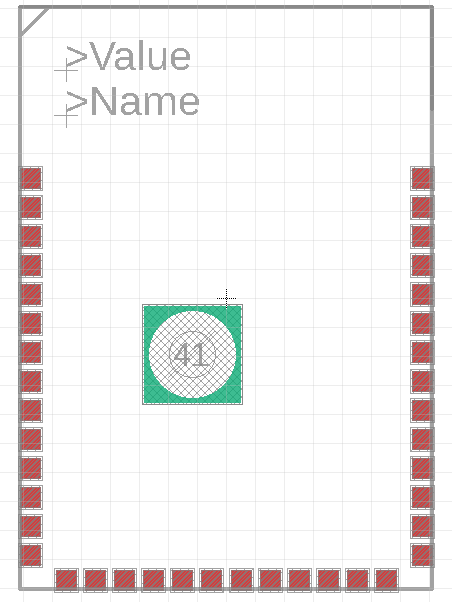
\includegraphics[width=0.7\textwidth]{imagenes/Capitulos/Cap04/ESP32S3HOLE.png}
    \caption{Imagen de la ESP32S3 modificada}
    \label{fig:ESP32S3HOLE}
\end{figure}

\newpage
\section{Diseño Esquemático}
Para el diseño esquemático se han importado todos los componentes a Eagle y se han creados distintas partes del sistema para posteriormente interconectarlas todas en el diseño final.

\subsubsection{Matriz del Teclado}
En esta parte se ha seguido el ejemplo básico que podemos ver en la figura \ref{fig:EjemploArrayTeclado} en el apartado de diseño. Donde se opta por una configuración de filas y columnas con su respectivo diodo para evitar \gls{Ghosting}. En la fase de diseño se decidió que iba a ser una matriz de 16*6 teclas únicas, una tecla especial individual y 13 teclas repetidas. La matriz finalmente queda como se muestra en la figura \ref{fig:MatrizTeclas}.

\begin{figure}[H]
    \centering
    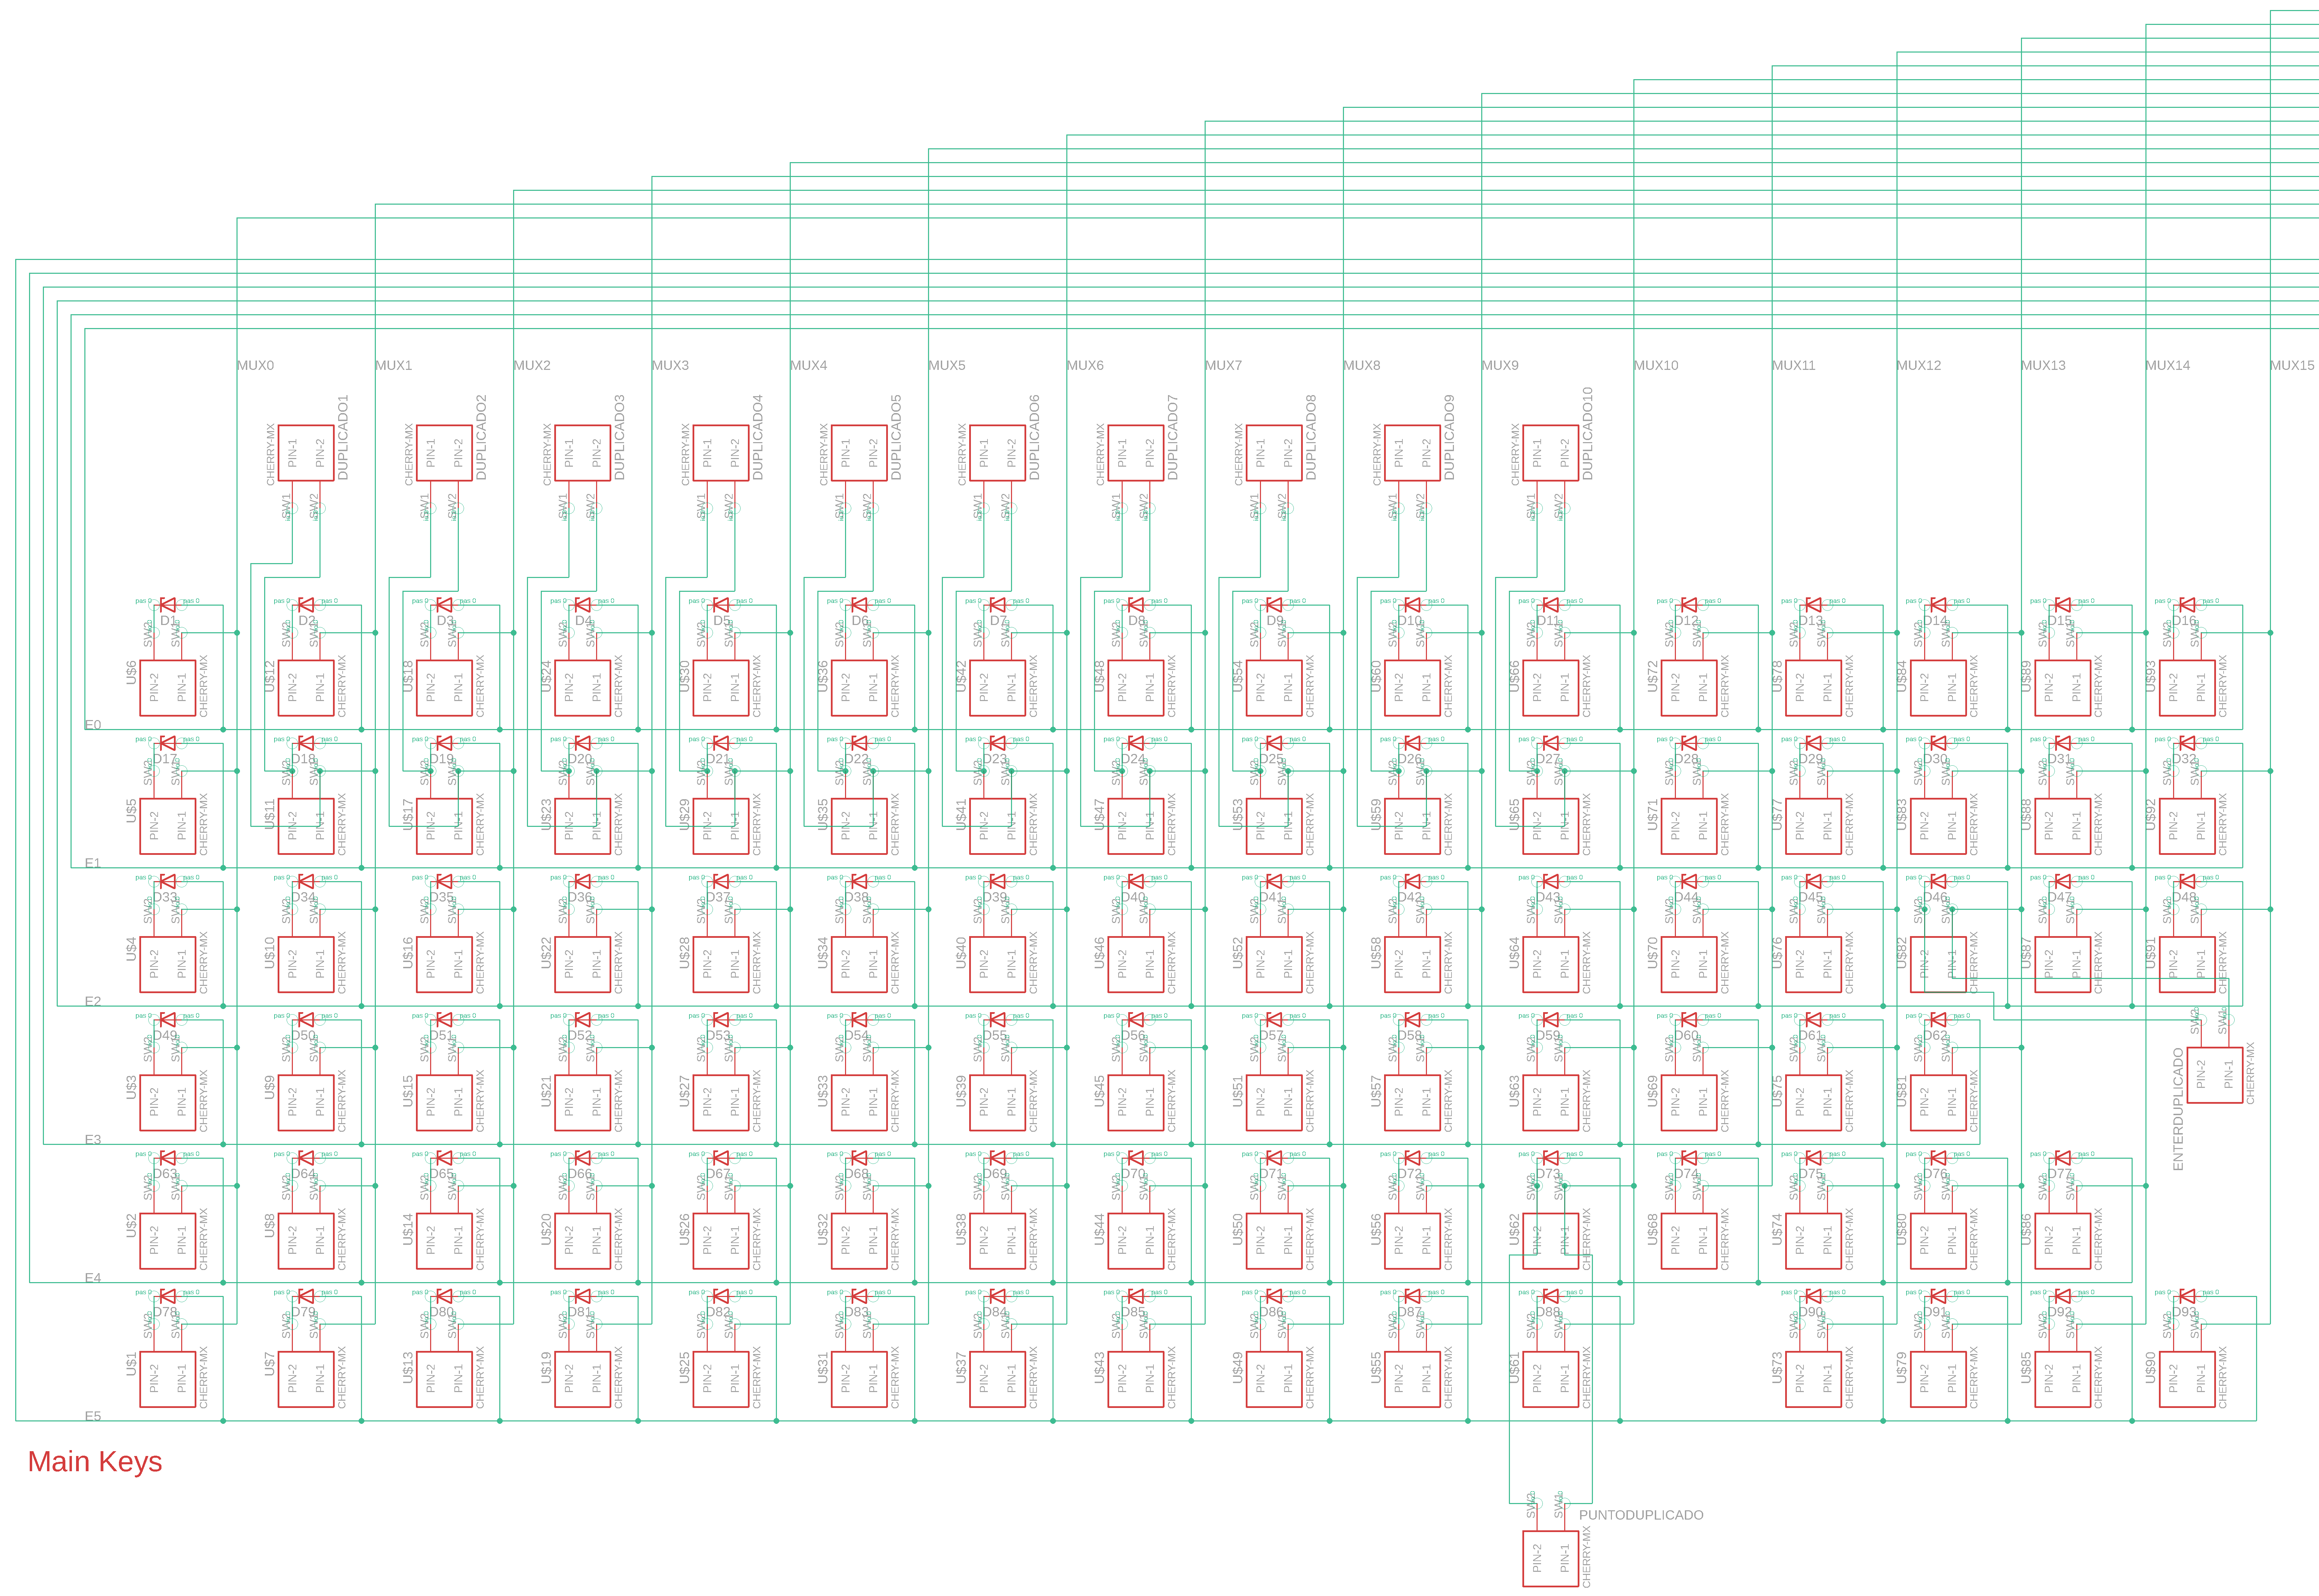
\includegraphics[width=1.0\textwidth]{imagenes/Capitulos/Cap04/MatrizTeclas.png}
    \caption{Matriz final de teclas}
    \label{fig:MatrizTeclas}
\end{figure}

\newpage
\subsubsection{\gls{Multiplexor}}
Esta parte se trata de las entradas y salidas del \glsnocase{Multiplexor} hacia la matriz y al microcontrolador. Esta parte es bastante sencilla como se puede apreciar en la figura \ref{fig:MuxImagenCircuito}.

\begin{figure}[H]
    \centering
    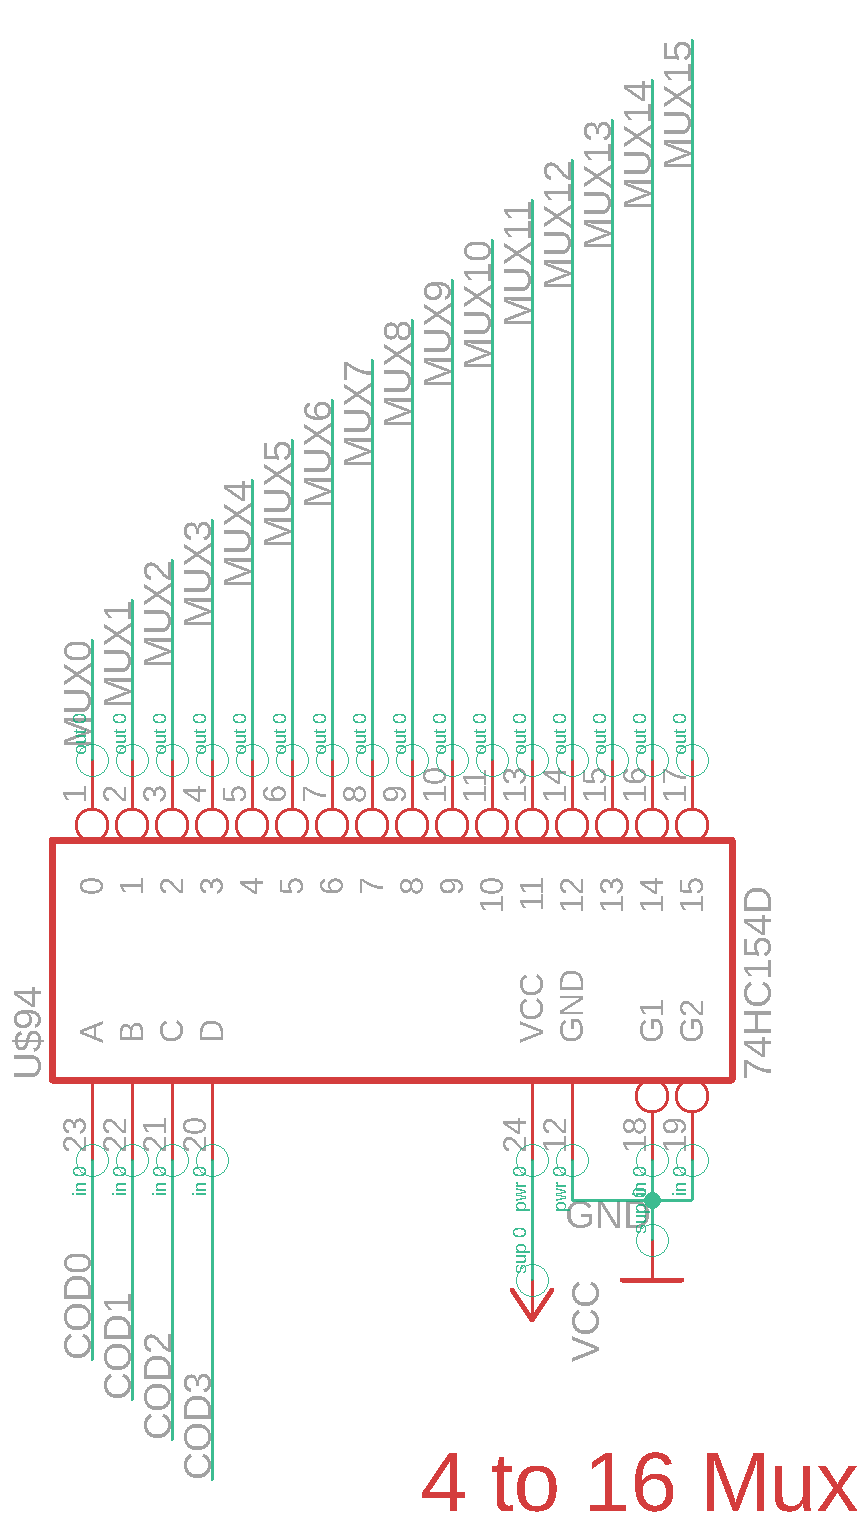
\includegraphics[width=0.6\textwidth]{imagenes/Capitulos/Cap04/Mux.png}
    \caption{\gls{Multiplexor} con todos los pines conectados a sus salidas/entradas}
    \label{fig:MuxImagenCircuito}
\end{figure}

\newpage
\subsubsection{Controlador Principal}
Esta parte del circuito es el chip principal (ESP32S3) junto con los botones necesarios para programarla en el momento de subir el firmware, las resistencias que mantienen la placa encendida y la única tecla especial. Todo se puede apreciar en la figura \ref{fig:ESP32S3Circuito}

\begin{figure}[H]
    \centering
    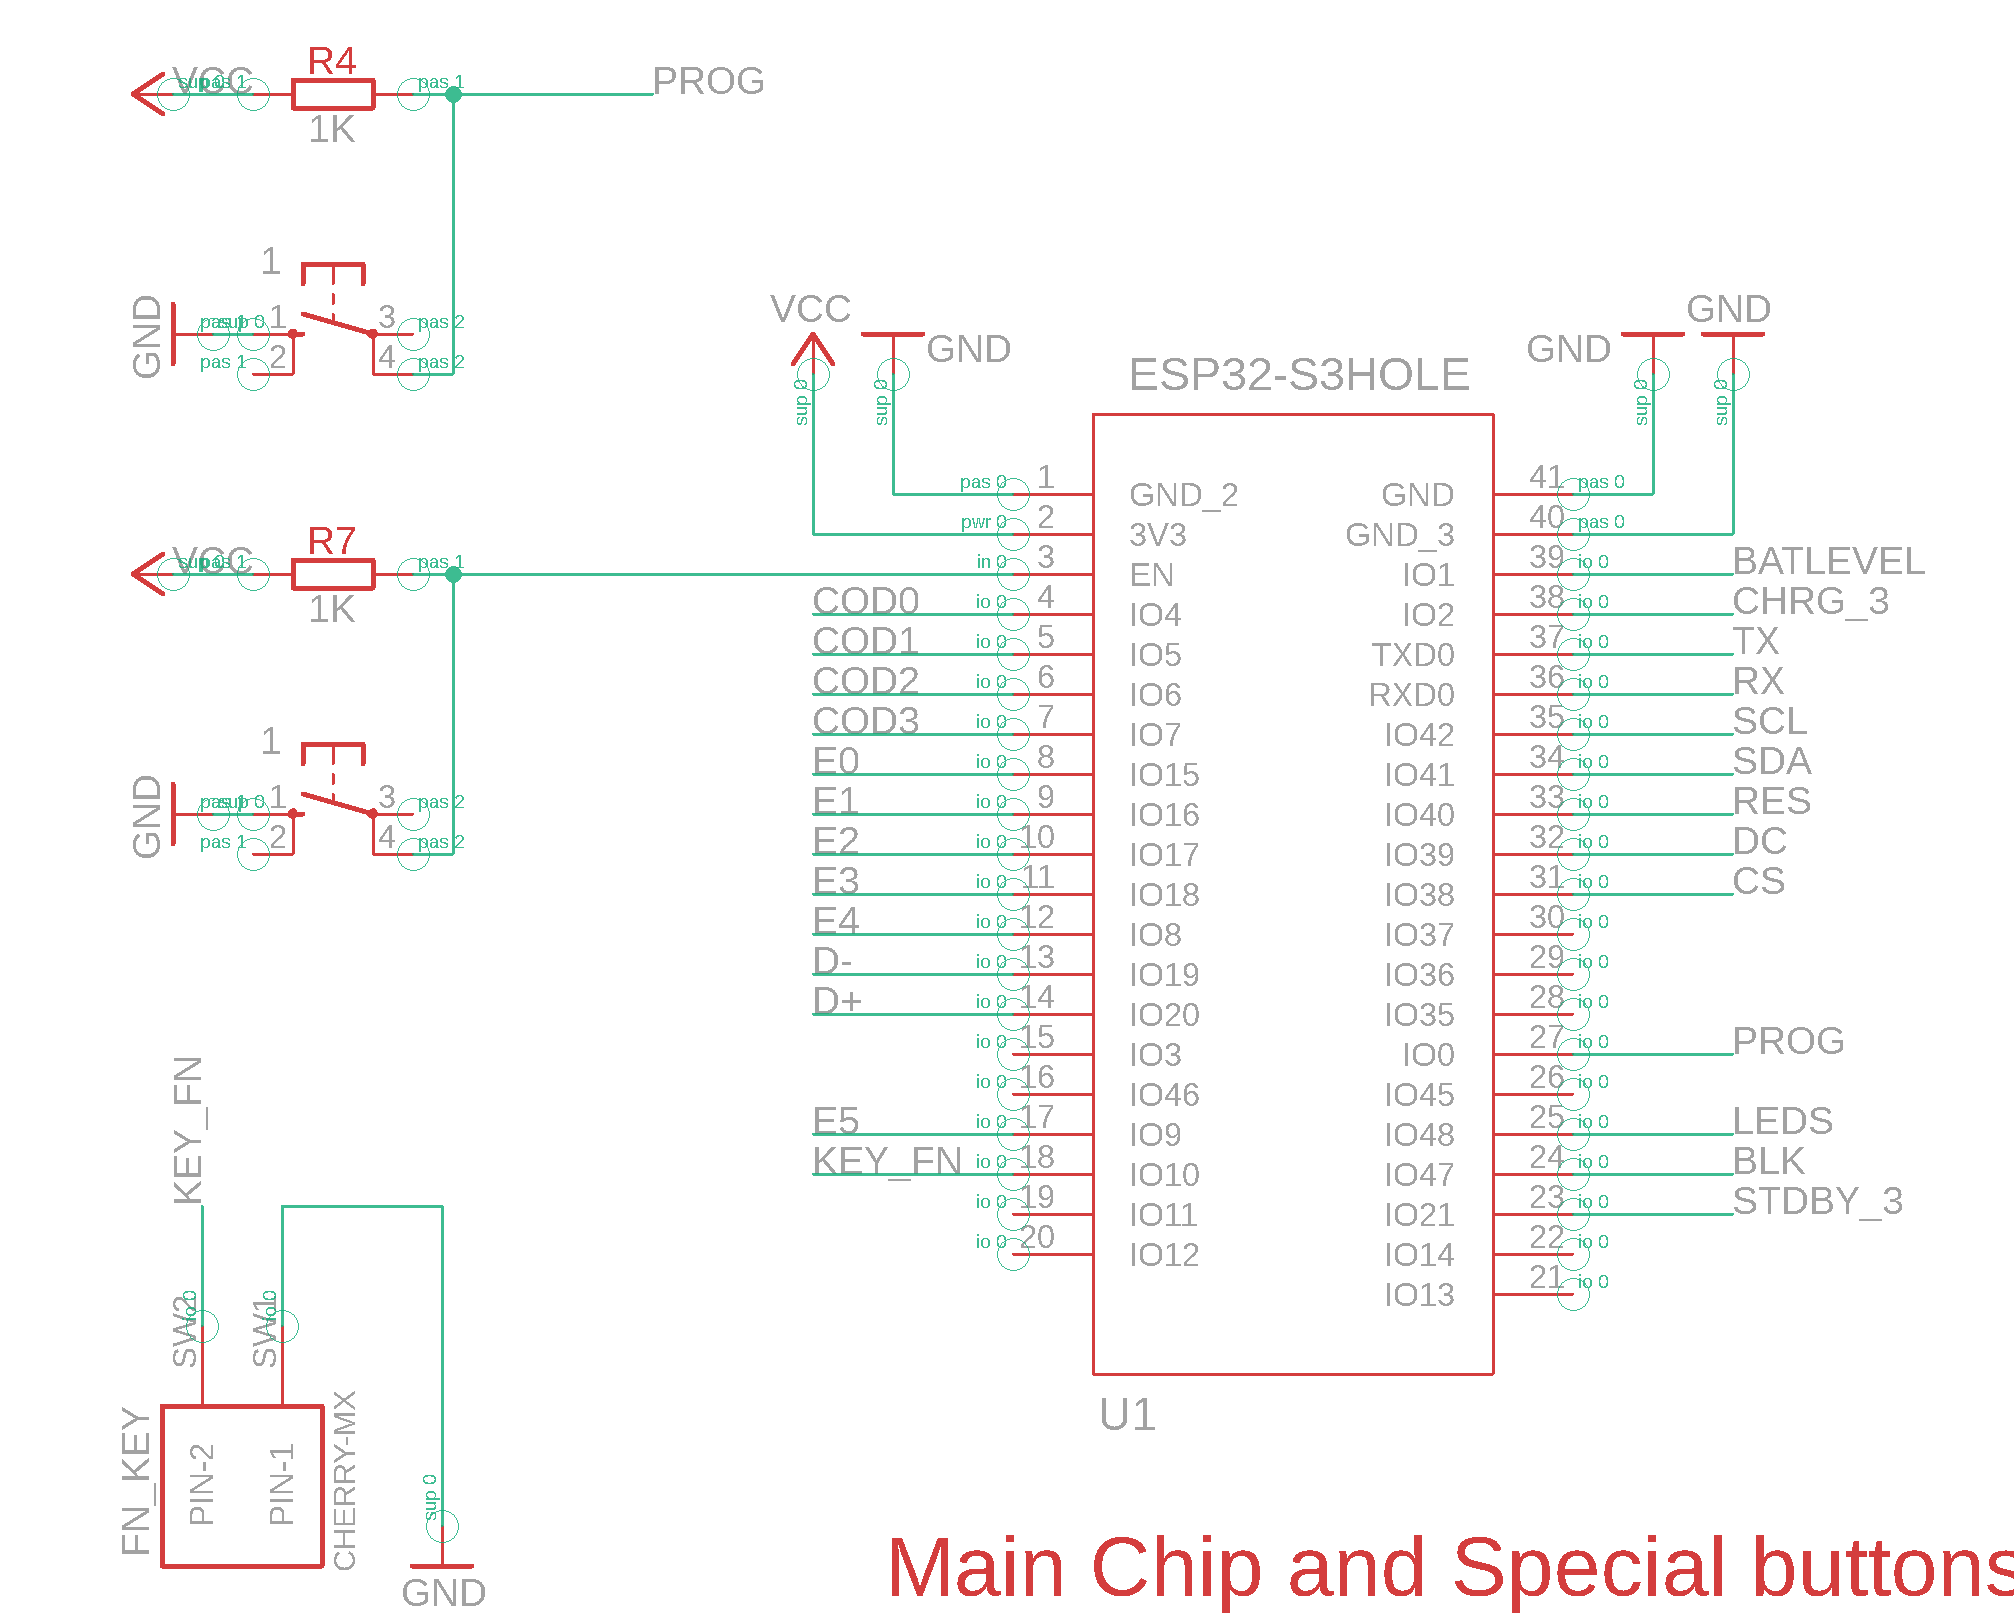
\includegraphics[width=1.0\textwidth]{imagenes/Capitulos/Cap04/CHIP.png}
    \caption{Microcontrolador principal ESP32S3 y tecla principal}
    \label{fig:ESP32S3Circuito}
\end{figure}

\newpage
\subsubsection{Bateria y alimentación}
Como este teclado tiene que soportar alimentación por batería a 4.2V, por USB a 5.0V y a 3.3V para el ESP32S3 es necesario un circuito que se encargue de estos voltajes, de proteger la batería y proteger todos los circuitos. Se puede ver el circuito encargado de esto en la figura \ref{fig:CircuitoBateriaAlimentacion}. Todo el diseño se ha hecho siguiendo el apartado \ref{InvestigacionSistemaBateria} y la figura \ref{fig:SchemeTP4056}.

\begin{figure}[H]
    \centering
    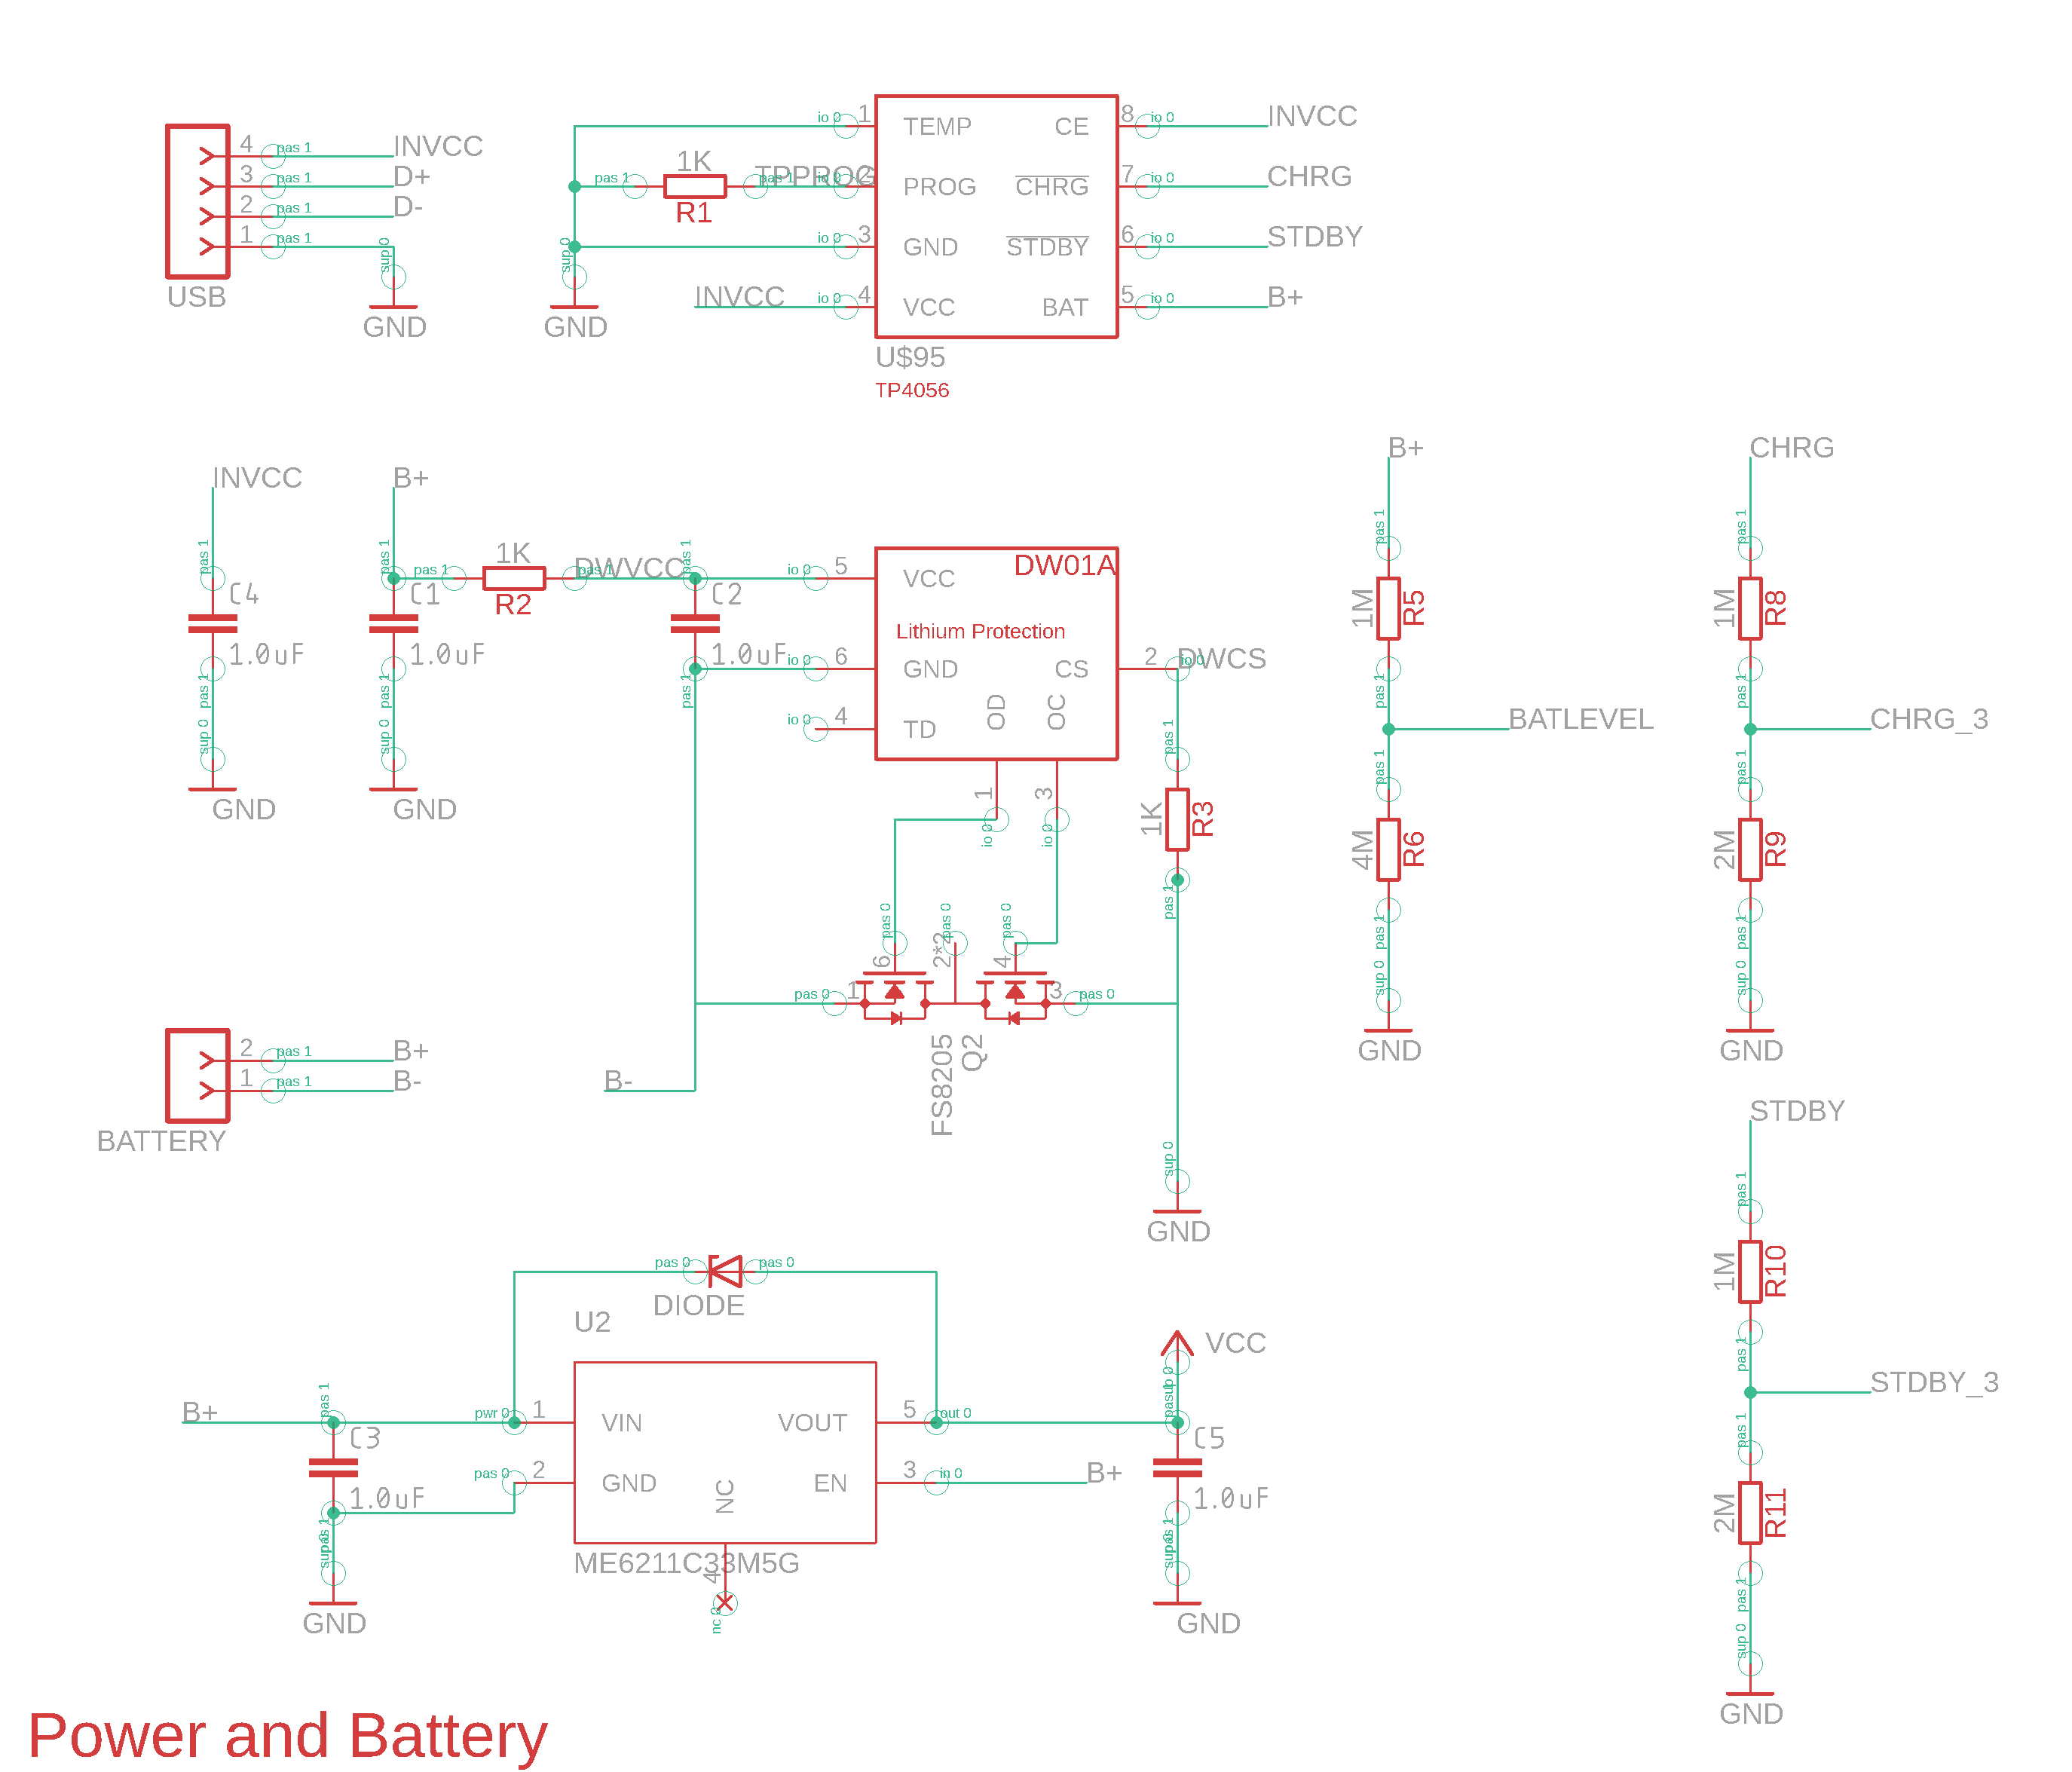
\includegraphics[width=1.0\textwidth]{imagenes/Capitulos/Cap04/Battery.png}
    \caption{Sistema de alimentación y protección del teclado}
    \label{fig:CircuitoBateriaAlimentacion}
\end{figure}

\begin{tcolorbox}[colback=red!11!white, colframe=red!50!white, title=Errores]
    Ver apartado de errores \ref{CorrienteInversa} y \ref{VoltajeRegulador} donde se explica por qué se ha añadido un diodo en la puerta del regulador de tensión.
\end{tcolorbox}

\newpage
\subsubsection{\gls{LED}S}
En la fase de diseño \ref{DiseñoLeds} se decidió que tuviera \glsnocase{LED}s, ya que eran faciles de programar y daban mucho juego. El apartado eléctrico de los \glsnocase{LED}s se puede observar en la figura \ref{fig:CircuitoLeds}.

\begin{figure}[H]
    \centering
    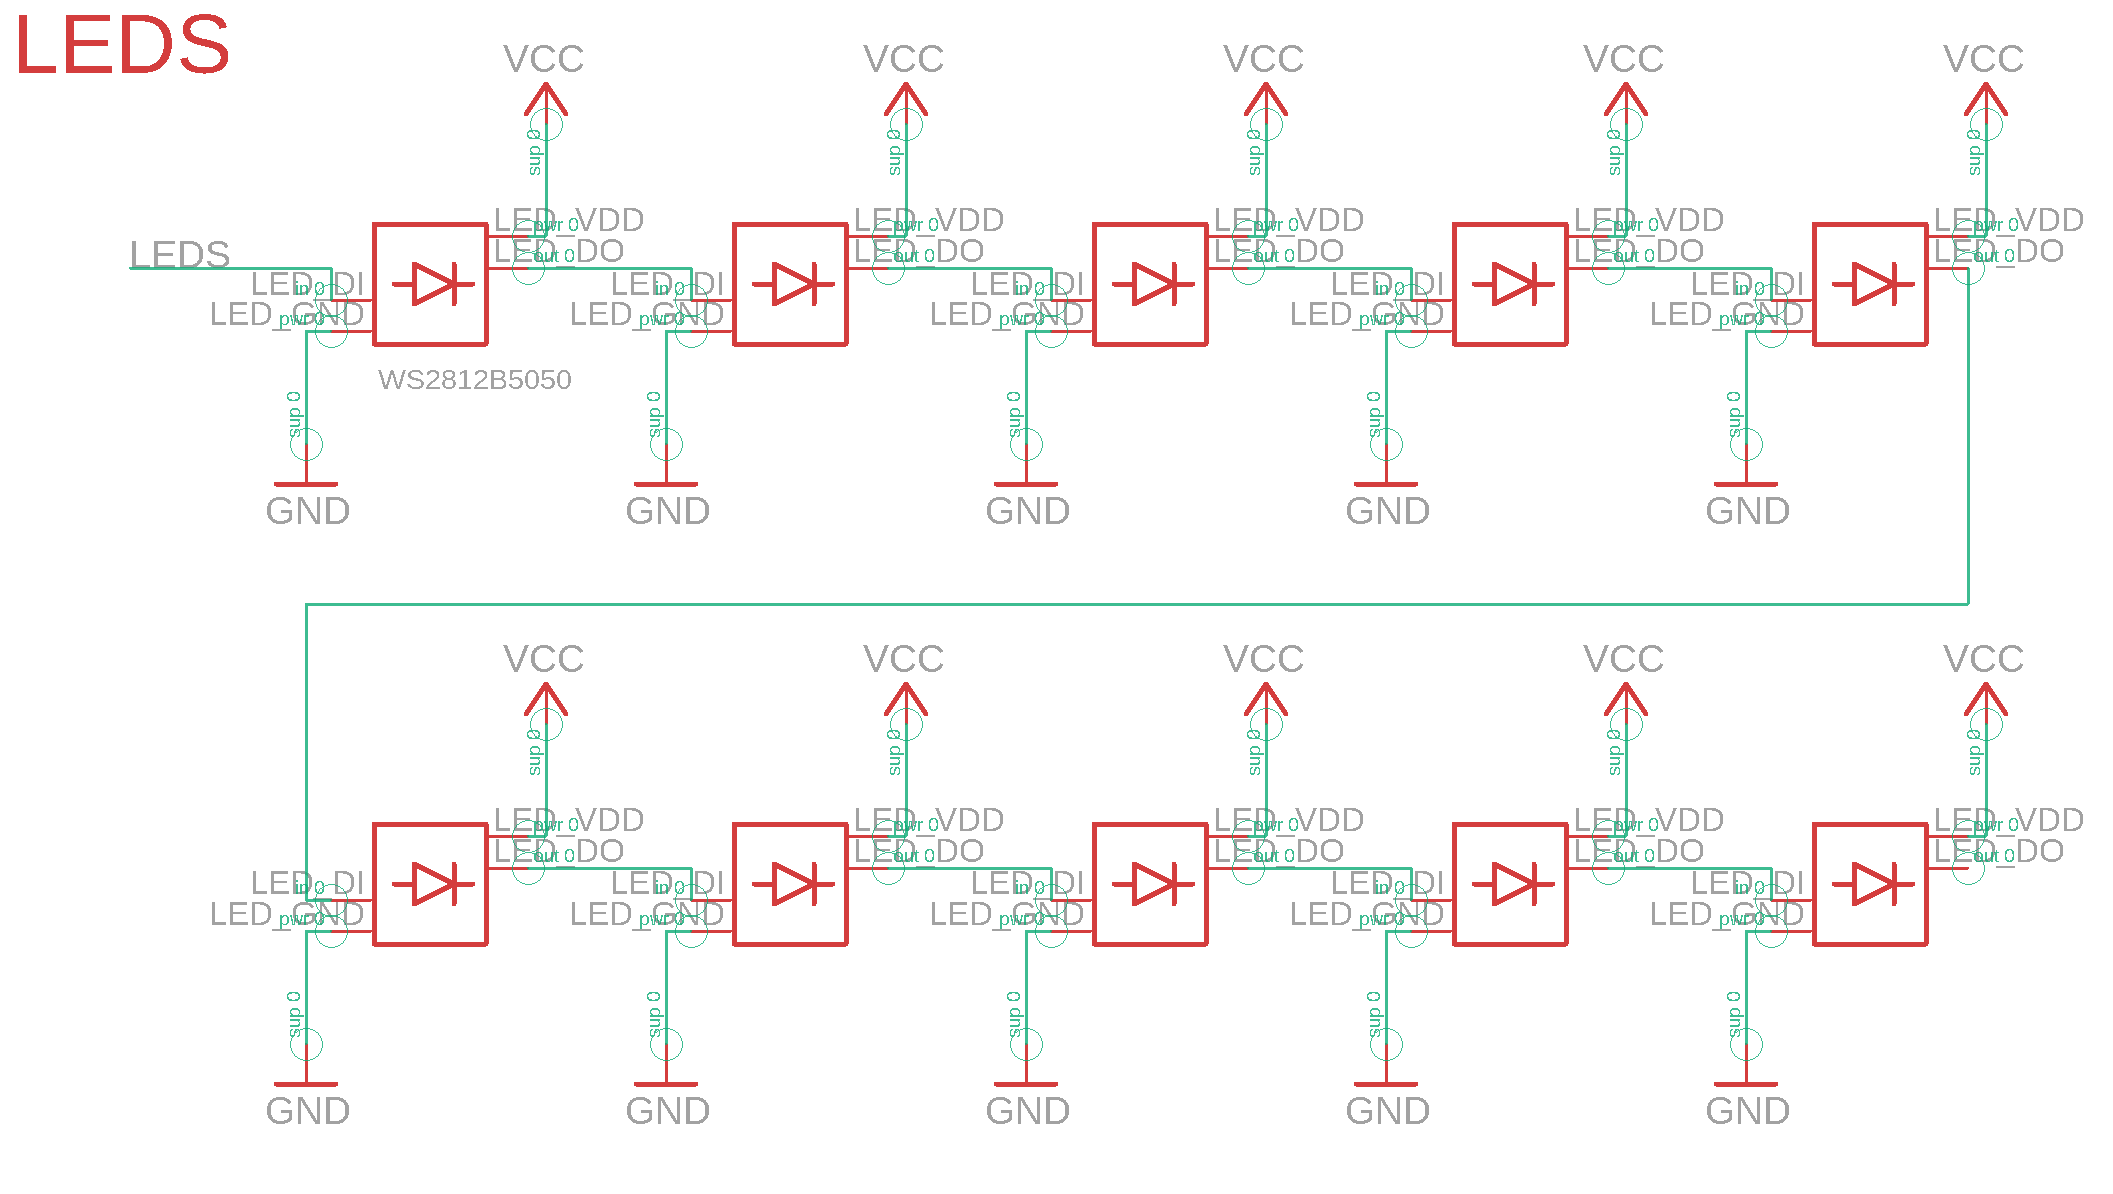
\includegraphics[width=1.0\textwidth]{imagenes/Capitulos/Cap04/LEDs.png}
    \caption{Sistema de \glsnocase{LED}s del teclado}
    \label{fig:CircuitoLeds}
\end{figure}

\subsubsection{Conectores para el teclado}
En el apartado de diseño \ref{DiseñoPantalla} aparecen los conectores que necesita la pantalla. Además se ha añadido otro conector más para poder programar el chip cuando este sea soldado en la placa. Por lo que como se observa en la figura \ref{fig:CircuitoConectores} nuestro teclado se compone de 2 conectores básicos.

\begin{figure}[H]
    \centering
    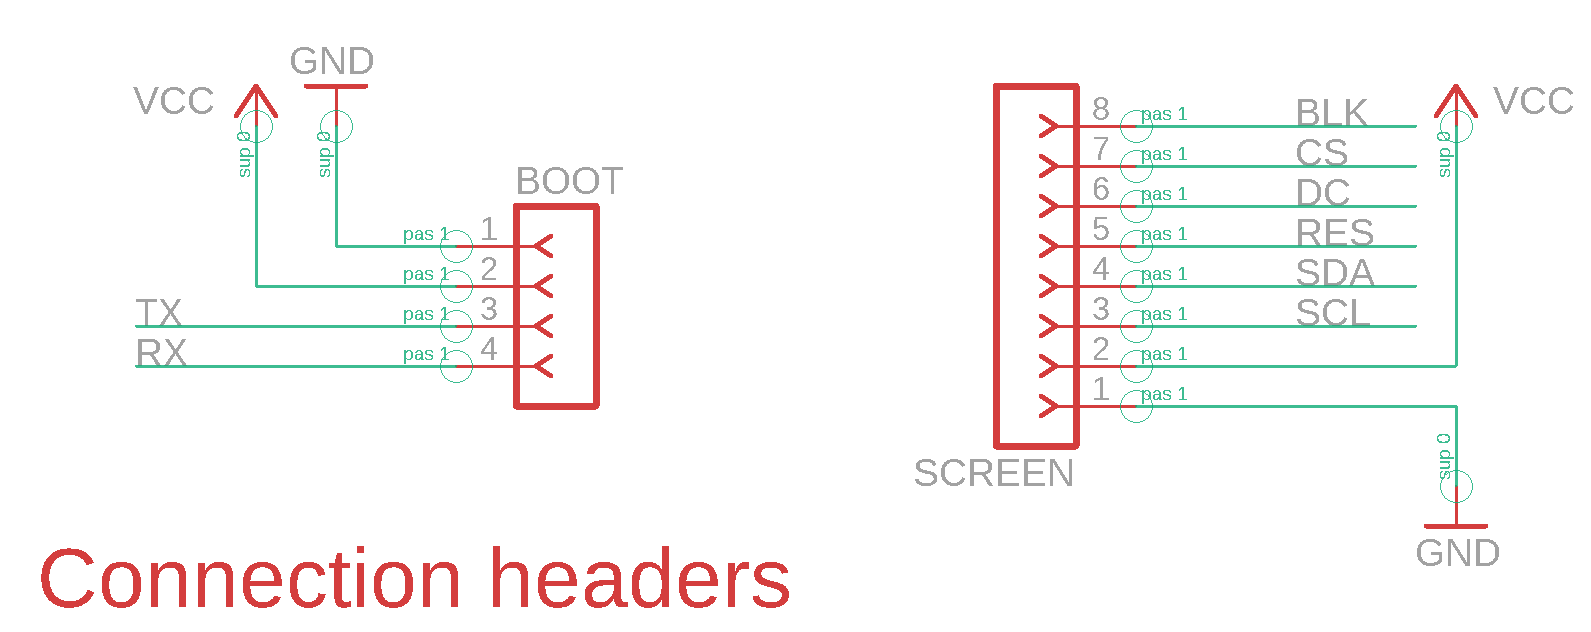
\includegraphics[width=1.0\textwidth]{imagenes/Capitulos/Cap04/Conectores.png}
    \caption{Conector de programación y conector de la pantalla TFT}
    \label{fig:CircuitoConectores}
\end{figure}

\begin{sidewaysfigure}
\centering
\includegraphics[width=\textheight]{imagenes/Capitulos/Cap04/Esquematico.png}
\caption{Esquema completo del circuito del teclado.}
\label{fig:CircuitoCompleto}
\end{sidewaysfigure}
